\chapter{Solution}\label{chap:solution}

This chapter presents the solutions to the problems exposed in Chapter \ref{chap:problem}. It explains the rationale behind them, as well as why they were preferred over their alternatives.

First, the general architecture is described, presenting the multiple components of the application. Afterward, each component is described in more detail, regarding its functionality and implementation.

\section{General Services Architecture}

This section describes the general architecture of the system. It is composed of multiple microservices, each handling a specific part of the problem. The main services are the ones dealing with the frontend application --- the website itself ---, the conflict handling, and the user reputation. Additional services are build in order to achieve a functional whole, and they will be described below. Fig. \ref{fig:services-arch} shows the system architecture design and how the services connect to one another.

All of these services are managed using Docker \footnote{https://www.docker.com/}. Each service is built in a Docker Container, allowing it to be easy deployed and replicted across machines for scalability and fault tolerance. It also ensures that every deployment is identical, no matter the host machine and environment it is deployed on.

Additionally, Docker Compose \footnote{https://docs.docker.com/compose/} is used to define how the different containers in a multi-container application should interact with each other, allowing us to start the application as one entity, instead of multiple isolated containers. It conveniently provides an DNS so that containers can reach each other by their service name.

Finally, a microservice architecture promotes isolation and independence of services, which in turn allows for easier development and testing. Different teams can work on each service, which has a single purpose, and they only need to agree on the interface and how they can communicate between them.

\begin{figure}[t]
    \begin{center}
        \leavevmode
        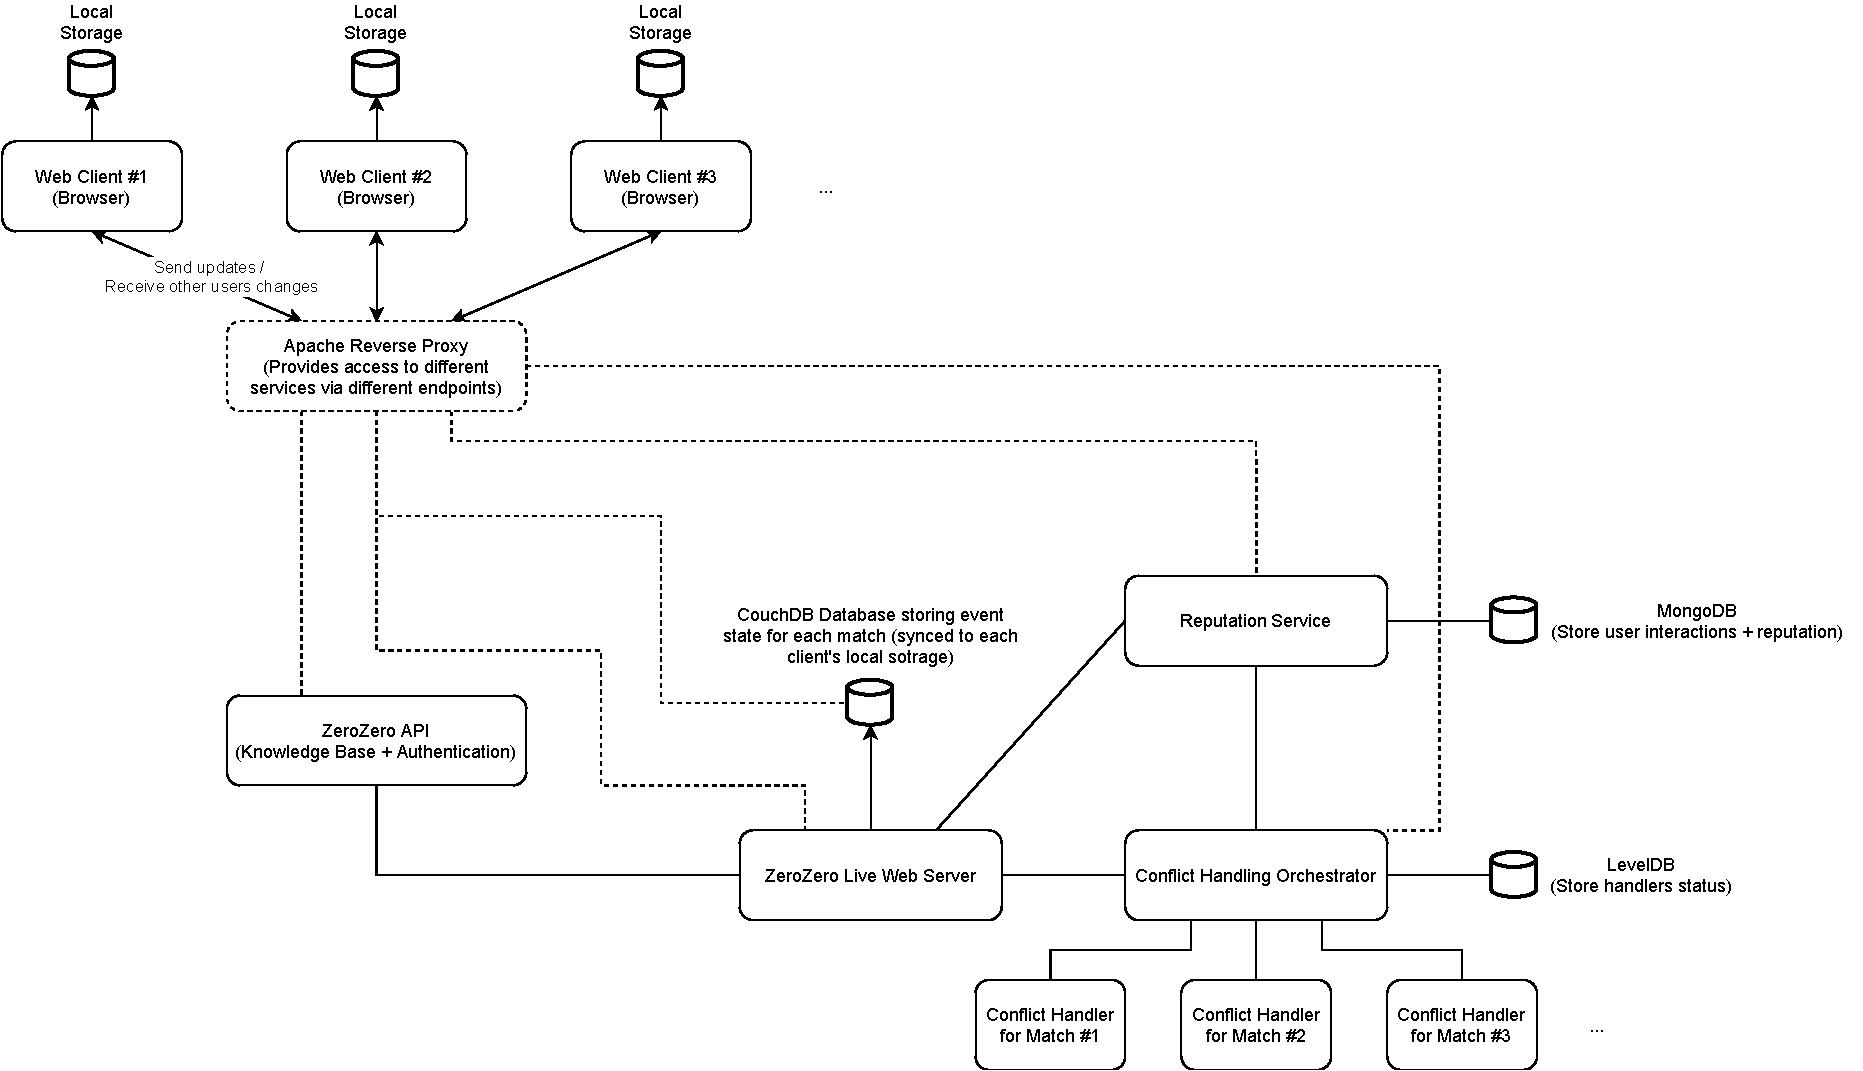
\includegraphics[width=0.8\textwidth]{zerozerolive-arch.pdf}
        \caption{Architecture design of the zerozero.live system}
        \label{fig:services-arch}
    \end{center}
\end{figure}

\subsection{Reverse Proxy}

In the zerozero.live deployment, only the 443 --- HTTPS --- port is exposed to the internet, thus, to expose multiple services, it cannot be done in multiple ports, at least not from the outside. Due to this, a reverse proxy is required to map each service --- and its specific port --- to an endpoint on the main domain zerozero.live:
 
\begin{itemize}
    \item \textbf{/} Redirects to the client application --- the website
    \item \textbf{/api} Redirects to a small proxy that communicates with the ZeroZero API
    \item \textbf{/db} Redirects to the CouchDB, holding the match events in real time
    \item \textbf{/manager} Redirects to the conflict handling services orchestrator, which monitors the conflict handlers for each match
    \item \textbf{/reputation-manager} Redirects to the reputation service, which registers the interactions and calculates the reputation updates for users 
\end{itemize}

\subsection{CouchDB}

CouchDB is a document-oriented, multi-master database, which allows for easy replication between nodes. This enables data to flow seamlessly from web browsers to the database and vice-versa, powering offline-first applications while being developer friendly, since the API that interacts with the local database --- powered by PouchDB --- is the same that interacts with the remote database --- CouchDB.

When compared to the previously analyzed alternatives, namely ShareDB and CRDT solutions such as Automerge, CouchDB is older and thus more \textit{battle tested} than the rest, while also having frequent releases --- the latest stable to date is from September, 2020. ShareDB has also been around for some time, since 2013, however, it offers a lower level alternative to conflict resolution using OT. It allows integration with any database and offers similar features to CouchDB, but I have found it difficult to program custom conflict resolution strategies, very much important to this work. From the three, Automerge is the youngest (2017), and it relies on a different approach to conflict resolution, based on CRDT. As it does not require a central server, it merges documents automatically and I could not find how to add custom resolution of conflicts, which led me to choose the CouchDB alternative.

It is based on documents which are JSON objects with at least an id and a revision identifier. CouchDB then uses this to detect conflicts --- if it has the same id, it may conflict --- and to resolve them. It works by creating a tree of documents, where the leaf nodes are the current winners, branches represent conflicting revisions, which are kept to be resolved by the application if needed. CouchDB will choose a winner automatically and deterministically, so that every client has the same version of the data. However it is possible to resolve the conflicts afterwards, by choosing a conflicting version as the winner, which appends a new node to the tree, after the previous winner, making the previously conflicting document the new leaf node, and thus the new winner for that document id.

Finally, this has the advantage of having a browser version, powered by PouchDB, which replicates the database to the browser's IndexedDB, and its API is the same as CouchDB's. This makes the application offline first, since all the changes are made to the local database, and continuously synchronized to the remote database.

\subsection{Conflict Handling}

After generating match events, conflicts may arise. The conflicting events are the ones whose documents share the same id. If we want documents to conflict, they cannot have unique ids, so the following schema was defined for each event id:
\begin{equation}
    eventMinute-eventMinuteExtra-eventCategory
\end{equation}

By having this schema, when any event from the same category is inserted, refering to the same game time as another, they will conflict. Event categories are defined in such a way that events from different categories do not conflict. Some category examples include goal related events (\textit{Goal}, \textit{Own Goal}, \textit{Big Scoring Opportunity}, etc.), card related events (\textit{Yellow Card}, \textit{Red Card}), or time events (\textit{Start Whistle}, \textit{End of 1st Half}, \textit{Final Whistle}, etc.)

This will ensure that we have a bascic conflict detection, however it can easily be noticed that even in the same category there may be events on the same minute: There can be a \textit{Big Scoring Opportunity} immediately followed by a \textit{Goal}, or even two \textit{Yellow Cards} for two different players, or even the same one.

To improve the experience, a conflict handler is needed, in order to automatically solve conflicts as best as possible.

\subsubsection{Conflict Handler}

As previously noted, the Conflict Handler will help resolve some existing conflict automatically, based on the conflicting events and the match context, in order to only rely on users to resolve pending conflicts as a last resource.

This is a Node.js process that will use PouchDB to connect to the remote CouchDB and listen for changes. It has two main responsibilities:
\begin{itemize}
    \item If the document does not have conflicts sync with ZeroZero API, by inserting, editing or deleting the event from their database, depending on the operation
    \item If the document has conflicts, try to resolve them according to the specified rules, by either deleting the conflict and keeping the current winner, deleting the conflict and adding it \textit{after} the previous winner, to choose it as winner, or keeping both documents, by deleting the conflict and adding a replicated document with a unique suffix added to the id so that it won't conflict again.
\end{itemize}

{\Huge TODO SHOW CONFLCIT RESOLUTION RULES (?)}

{\Huge falar das chamadas ao rep service disagree vs explicit agree}


\subsubsection{Conflict Handling Orchestrator}

In order to have multiple handlers at once, which is needed as there may be multiple matches happening at the same time, one needs to have a controller that handles their initialization, manages their status and stops them once they are not needed anymore.

That is the responsibility of the Conflict Handling Orchestrator. It is a simple Node.js application that exposes an HTTP API, that lets us initialize a conflict handler for a given match, list active handlers, stop a conflict handler for a given match, and \textit{kill} any \textit{zombie} handler references that might be left over after a crash. The state of the handlers is kept in a LevelDB\footnote{https://github.com/google/leveldb} database, which is a simple key-value database. Each record will have the match id as the key and the value is an object containing the PID of the handler process for that match, as well as the timestamp of when the handler was started.

Even though the orchestrator is the parent process of the conflict handlers, in case the conflict handler process fails, the orchestrator is independent enough that it won't terminate as well. If the orchestrator itself fails for some reason, it is built to auto-restart instead of making the docker container restart, which would make it lose context and terminate all other processes, including child conflict handlers. This is why information about the handlers is kept in a separate database, instead of in-process memory, so that the orchestrator can recover all of it in case of failure.

\paragraph{POST /initConflictHandler/:matchId}
This endpoint launches a child process running a conflict handler for the specified match, as described in the previous subsection. It is made in such a way that it won't allow the launch of multiple handlers for the same match simultaneously. After a specified timeout, the child process is killed, to avoid wasting resources on finished matches.

\paragraph{POST /stopConflictHandler/:matchId}
This endpoint terminates a process associated with the given match.

\paragraph{GET /active-handlers}
This endpoint returns a list of active match conflict handlers, together with their respective PIDs.

\paragraph{POST /cleanup-zombies}
This endpoint will verify that every stored match handler is actually running. If not, it will update the database. This is important because after some failure, conflict handlers might not be running as the database shows, and this endpoint will restore the truth.

\subsection{Reputation Service}

In order to aid the automatic conflict resolution, in many cases, the reputation of the users will be used to determine which event to choose as the conflict winner. This is only done for conflicts that are not critical. For any important conflict --- such as \textit{Goal from team A} vs. \textit{Goal from team B} --- it is left for users to resolve manually on the UI.

The Reputation System is based on the fact that people that input conflicting events disagree with each other, as well as who edits or deletes an event. Every time a user receives an event from someone, they implicitly agree with it, until they act to mark disagreement, executing any of the actions described before. Finally, users can explicitly agree with each other, by inputting conflicting events, that are exactly the same i.e., if two users report a goal from team A at the same time, they are not disagreeing with each other, but rather agreeing. This is considered a more \textit{powerful} agreement, since they both explicitly inputted the event, instead of just waiting for someone to do it and passively reading it. These are the three interaction types that are regsitered by the reputation service.

The Reputation Service is a Node.js microservice that exposes an HTTP API, and uses a \mbox{MongoDB} database to persistently store data. It has endpoints to register interactions between users and inputs and another endpoint to calculate reputation updates after a specific match interactions.

The database will store the interactions, which are documents containing $matchId$, $eventId$, $userId$, $eventOwnerId$, $isProcessed$, $interactionType$. $matchId$, $eventId$, and $userId$ uniquely identify an interaction and are used to prevent the same user from registering multiple interactions for the same event. Additionally, there are checks in place so that a user cannot register interactions for an event they have inserted. $isProcessed$ is a boolean flag that marks the interaction as processed by the reputation calculation, so that it is not used multiple times when calculating reputation updates. Finally, the $interactionType$ defines the type of interaction, which affects the reputation update calculation, e.g., $Agree$, $Disagree$, $Explicit Agree$

Additionally, the database has another collection to store the user and their respective reputations, to be used in the conflict resolution. Each document has $userId$, $reputation$ and $updatedAt$ fields. The $reputation$ represents the numerical value of the reputation of the user with id $userId$, and the $updatedAt$ field is used to calculate the reputation decay --- the more time passes after the previous reputation calculation, the more its reputation will decay due to inactivity.

{\Huge WHY MONGO}
{\Huge REP calc algorithm, maybe no endpoint respetivo?}
{\Huge falta endpoint de get rep from user - para ser usado no conf.res}

\paragraph{POST /:matchId/:eventId/:eventOwnerId/:userId/agree}

\paragraph{POST /:matchId/:eventId/:eventOwnerId/:userId/disagree}

\paragraph{POST /:matchId/:eventId/:eventOwnerId/:userId/explicit-agree}

\paragraph{POST /:matchId/updateRep}

{\Huge Talk about constant values choice e graficos com predicts e exemplos de user behavior}

\subsection{Web Application (Frontend)}

